\chapter{Evaluation}\label{chap:evaluation}
The following section utilizes the simulative implementation of the Blockchain Gossip Model to evaluate the relationship between selfish mining and networking effects. Additionally, the model will be validated against data provided by \gopalan and real world data of the Bitcoin system.
\section{Simpy Blockchain Simulator}
The core implementation is based on simpy~\cite{simpy}. Simpy is a discrete event simulator written in python. As a result the Simpy Blockchain Simulator is also written in python. 
The Selfish Rumor Model consists mainly of four parts. 
\begin{itemize}
\item Networkgraph representation
\item Blockchain representation
\item Block Arrival Process representation
\item Communication Process representation
\end{itemize}
The network graph is represented by an adjacency matrix. The blockchain representation is a set of blocks and a set of edges for each peer, which are developing over time. The block arrival process and the communication process are modeled as a Poisson process~\cite{poisson}. This is mirrored in a Simpy process with an exponentially distributed interarrival time between scheduled events.
On each event of the block arrival process a block arrives at a random peer. This means that the event triggered by the block arrival process updates the blockchain datastructure accordingly.
At each event of the communication process $T_i$ a peer $p_i$ tries to update a certain peer $p_j$ according to the epoch associated with the event. This results in a comparison between the datastructures associated with $p_i$ and $p_j$ and an update of $p_j$, if it is possible.

Even though the basic implementation is simple, there are various parameters which influence the system behavior greatly. The following list shall give an overview:
\begin{itemize}
\item Average of interarrival times - This is the rate of block arrival process and communication process trigger events. 
\item Topology of the network graph - The network resulting from the adjacency matrix has a great influence on the behavior of the system.
\item Block selection - In a scenario, where multiple blocks could be transferred from one peer to another, one block has to be selected. How this block is selected influences system baviour.
\item Network size - This is the number of peers.
\item Mining power distribution - The mining power distribution influences the peer selection. Peer selection is the process of deciding which peer gets the new block once the block arrival process triggers an event.
\end{itemize}
The above discussed parameters can be modified in order to capture different systems.

\section{Validation of the Simpy Blockchain Simulator}
In the following section the Simpy Blockchain Simulator is validated against synthetic experiments published by the original authors of the blockchain gossip model. Additionally real world data from Bitcoin will be additionally used to validate the legitimacy of the Simpy Blockchain Simulator. This will lay the fundamant for further analysis concerning the network and selfish mining. 
\subsection{Validation of Simulator against \gopalan}\label{gopalananalysis}
In the synthetic data experiments of \gopalan~  they analyze the the network for 10, 20 and 30 peers. The network topology is a complete graph. Thus, the adjacency matrix is the unit matrix. 
The authors introduce four key metrics to analyze the system. Those are 
\begin{itemize}
\item Time to Consistency --- The average time an inconsistent system needs to reach a state of consistency
\item Cycle Length --- The sum of the average time to consistency and the average of the time the system stays consistent
\item Consistency Fraction --- The average fraction of peers that are consistent at each point in time
\item Age of Information --- The average number of blocks an average peer is away from the consistency state
\end{itemize}
All metrics mentioned above refer to the term consistency. The Consistency is defined as $B_G(t)$~\ref{unisondef}, the unison of all blocks produced by the block arrival process $A$.
In order to evaluate to capture the same system, that was analyzed by the authors, the parameters are setup similar.
These metrics can be used to verify whether the Simpy Blockchain Simulator is achieving similar numbers to the implementation of \gopalan . As for the parameter setup the interarrival time of the communication process is set to $1s$. The interarrival time of the block arrival process is a variable. The network topology is a complete graph. In a scenario, where multiple blocks could be transferred from one peer to another the block with the lowest index number is chosen. The network size is set to 10, 20 and 30 peers accordingly. The mining power distribution is uniform.

\begin{figure}[h]
	\begin{subfigure}[b]{0.5\textwidth}
		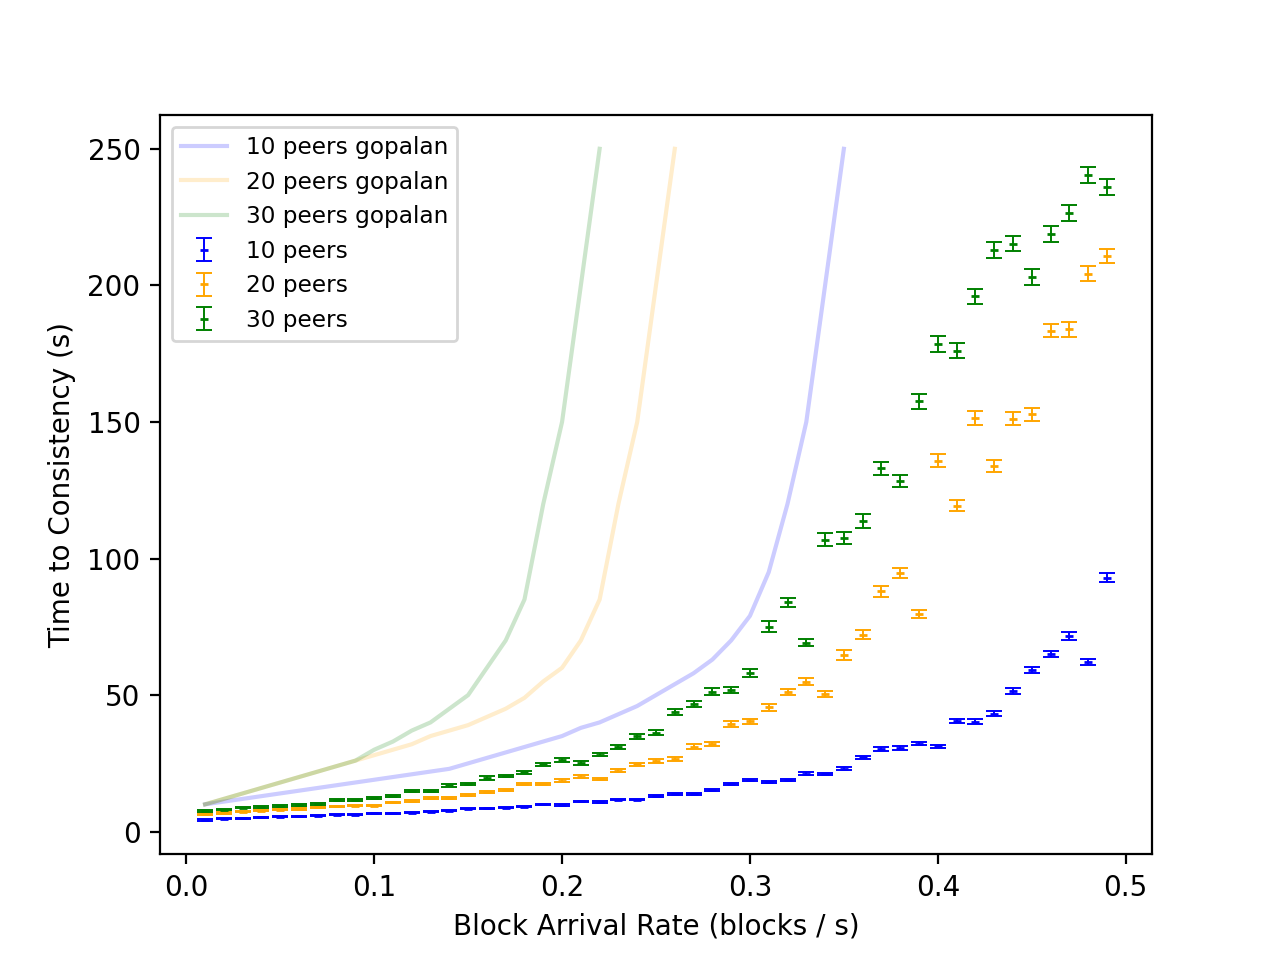
\includegraphics[width=\textwidth]{figures/gopalan_figures/time_to_consistency.png}
		\caption{ Time to Consistency}
		\label{fig:gopalan_ttc}
	\end{subfigure}
	\hfill
	\begin{subfigure}[b]{0.5\textwidth}
		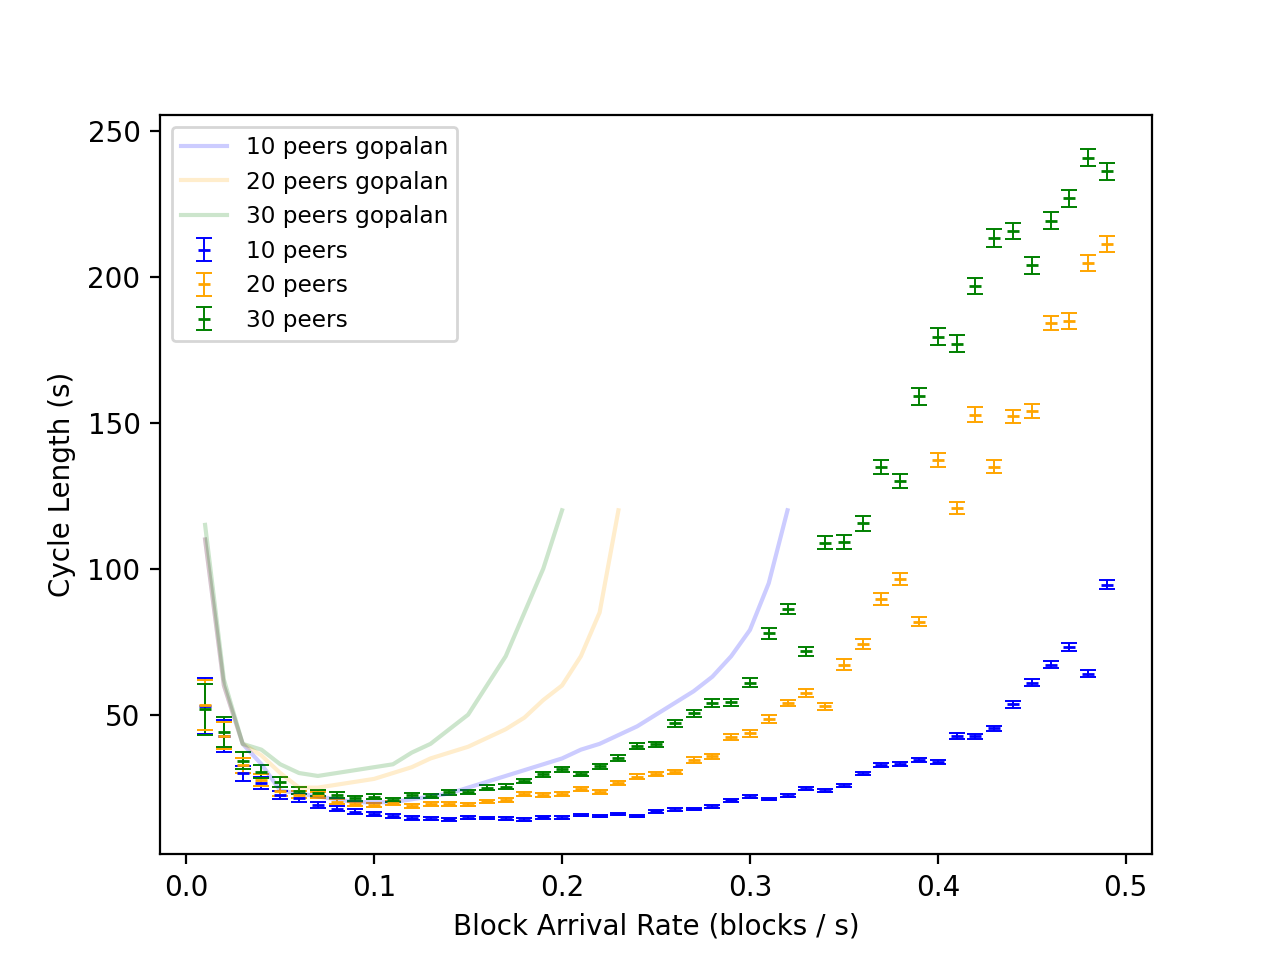
\includegraphics[width=\textwidth]{figures/gopalan_figures/cycle_length_avg.png}
		\caption{ Cycle Length}
		\label{fig:gopalan_cl}
	\end{subfigure}
	\hfill
	\begin{subfigure}[b]{0.5\textwidth}
		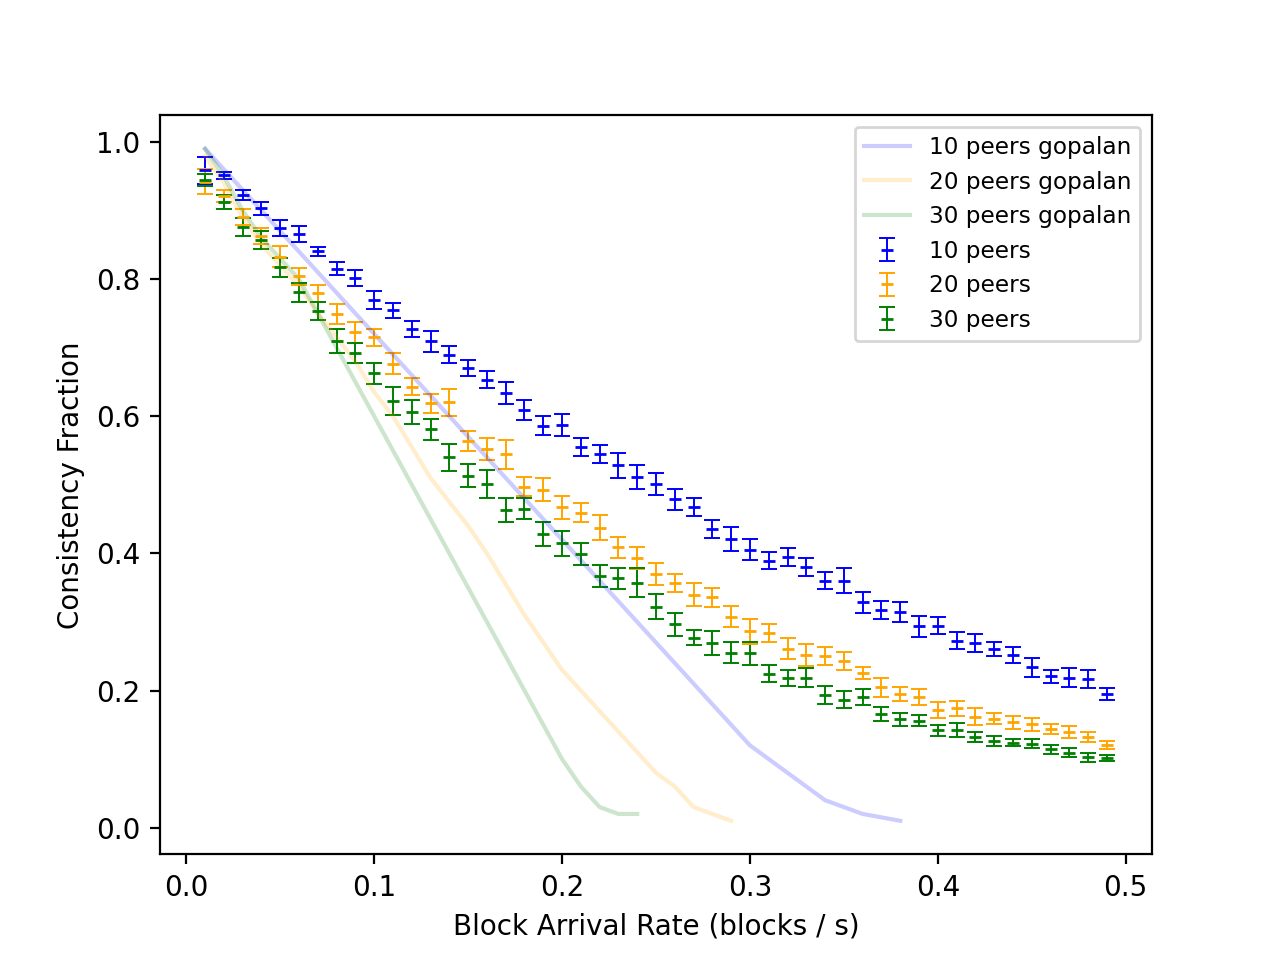
\includegraphics[width=\textwidth]{figures/gopalan_figures/consistency_fraction.png}
		\caption{ Consistency Fraction}
		\label{fig:gopalan_cf}
	\end{subfigure}
	\hfill
	\begin{subfigure}[b]{0.5\textwidth}
		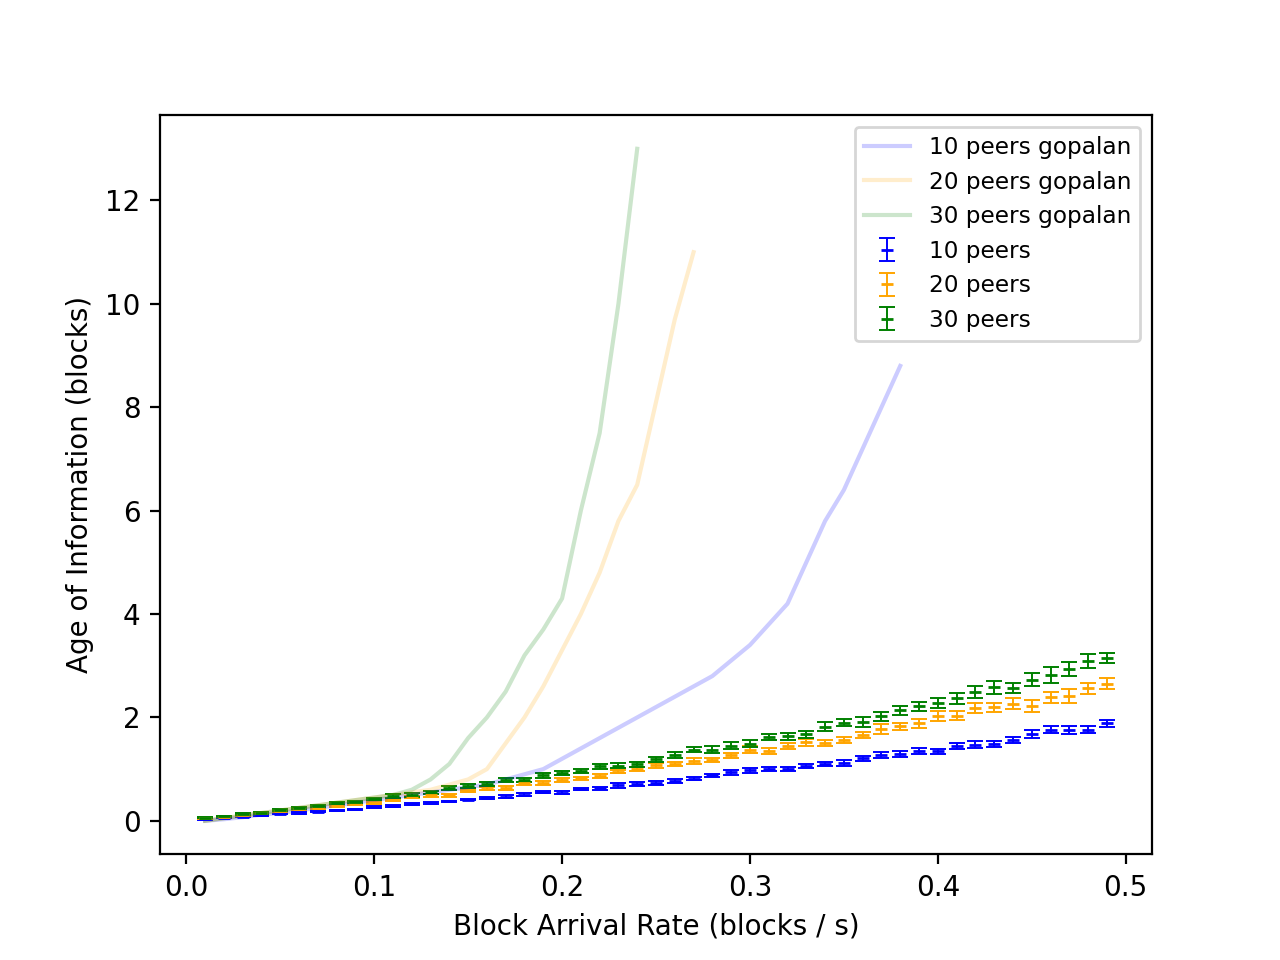
\includegraphics[width=\textwidth]{figures/gopalan_figures/age_of_information.png}
		\caption{ Age of Information}
		\label{fig:gopalan_aof}
	\end{subfigure}
	\caption{Comparison between Simpy Blockchain Simulator and values produced by \gopalan}
\end{figure} 

The metrics of time to consistency and cycle length are very closely related, because both rely on the time the system needs to reach consistency.
Figure~\ref{fig:gopalan_ttc} and Figure~\ref{fig:gopalan_cl} show this close relationship. Additionally the comparison between the Simpy Blockchain Simulator shows a very similar tendency in both metrics. Especially in Figure~\ref{fig:gopalan_ttc} it is observable that the curve has the same shape, only flatter. Figure~\ref{fig:gopalan_ttc} shows that peernumber and block arrival rate are proportional to the average time to consistency. Since cycle length is the sum of the average time to consistency and the average of the time the system stays consistent the same behavior can be observed in Figure~\ref{fig:gopalan_cl}. Additionally Figure~\ref{fig:gopalan_cl} shows that for very small numbers for the block arrival rate the cycle length increases again. When the system has a low block arrival rate the system tends to stay longer in a state of consistency, which is due to the fact that the idle time increases.

Consistency fraction and age of information are both metrics measuring the consistency of an average peer. The consistency fraction is the fraction of peers, which have a blockset equal to $B_G(t)$~\ref{unisondef}. For both the simulation results by \gopalan~ and the Simpy Blockchain Simulator we can observe, that the consistency fraction decreases with an increasing blockrate and peer number. While the exact numbers do differ, similar shapes can again be observed.
The age of information metric analyzes how much an average peer differs from $B_G(t)$~\ref{unisondef}. It showcases an increase for an increasing blockrate and peer number.

The differences indicate that information spreads faster in the Simpy Blockchain Simulator. After a brief discussion with \gopalan~, they confirmed that this might be due to the fact, that in the simpy version communication processes are handled truly concurrently.	

\subsection{Validation of Simulator against Bitcoin data}
This section validates the model against a real world blockchain system, the Bitcoin network. The Selfish Rumor Model implements an abstract network model of blockchain systems, simulating block creation and block propagation.
Researchers of the Karlsruher Institut für Technologie \cite{BitcoinNetworkMonitor} monitor the Bitcoin network and obtain data of, for example, the current block propagation delay distribution. Since the model can be used to analyze blocks and their propagation, the current block propagation delay distribution is a suitable metric to compare the Selfish Rumor Model against the real world system.\\
Bitcoin block propagation has two distinct characteristics. The distribution has a high peak at around $~400ms$ and a significant long tail, with block delays going up to $30s$. Since the whole dataset contains many outliers, $5\% $ of the largest delays are filtered out. This data is then used to match parameter setups of the Selfish Rumor Model against Bitcoin and find setups offering a similar block propagation.\\
To achieve a similar block propagation one can mainly analyze the topology of the network graph and the communication process rate.
The current Bitcoin network has an unknown topology. The original protocol described an algorithm, where a peer tries to maintain at least 8 connections. This would result in a random regular graph as network topology. However, analysis of the Bitcoin network comes to a different conclusion.
For example \cauth{baumann2014exploring} found strong indicators for a scale-free degree distribution.
Additionally, the FIBRE network and Compact Blocks were introduced to enable faster block propagation~\cite{measurement}. This results in a network topology, which cannot be captured by single graph representation.\\
Since the Selfish Rumor Model uses one single graph representation the objective is to utilize a topology and minimize the Root-Mean-Square-Error compared to Bitcoins block propagation. Therefore, either a regular random graph or a scale free graph should be chosen as a network topology for the Selfish Rumor Model. 
\begin{figure}[h! t]
	 \begin{subfigure}[b]{0.48\textwidth}
		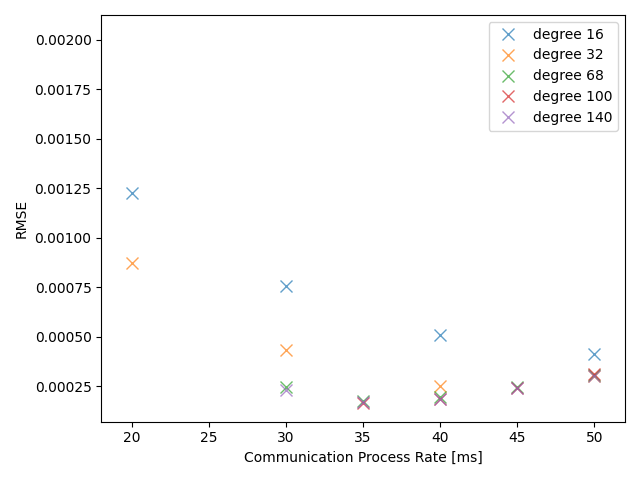
\includegraphics[width=\textwidth]{figures/RMSE_95.png}
		\caption{Root-Mean-Square-Error between Selfish Rumor Model regular-random Graph and Bitcoin}
		\label{fig:RMSE}
	\end{subfigure}
	\hfill
	\begin{subfigure}[b]{0.48\textwidth}
		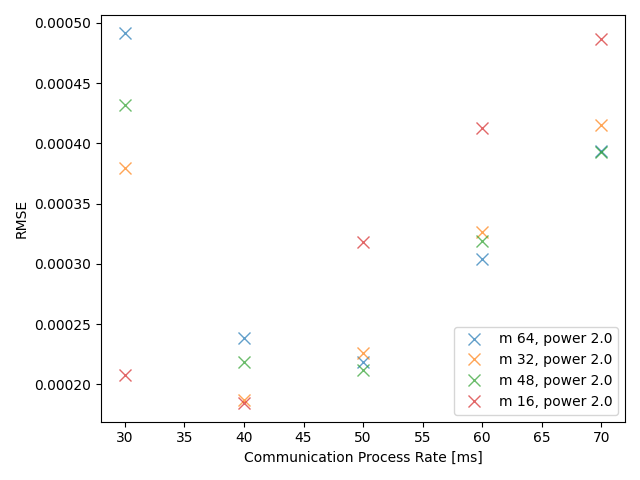
\includegraphics[width=\textwidth]{figures/RMSE_95_barabasi.png}
		\caption{Root-Mean-Square-Error between Selfish Rumor Model scale-free Graph and Bitcoin}
		\label{fig:RMSEBar}
	\end{subfigure}
	\hfill
	\begin{subfigure}[b]{0.48\textwidth}
		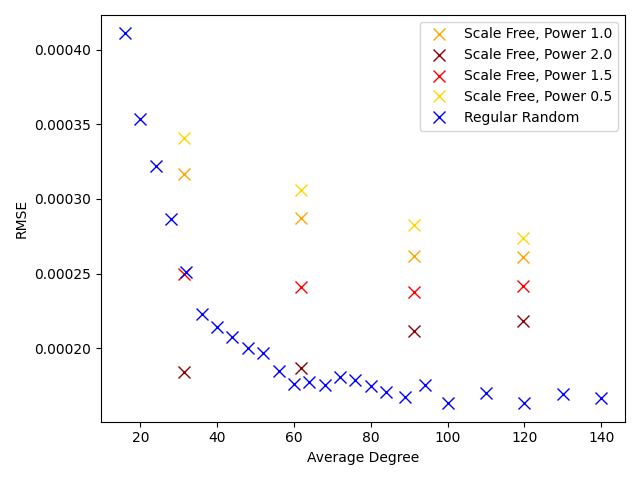
\includegraphics[width=\textwidth]{figures/rmse_min.png}
		\caption{Minimum RMSE value in random-regular graph and scale-free graph}
		\label{fig:minRMSE}
	\end{subfigure}
	\hfill
	\begin{subfigure}[b]{0.48\textwidth}
		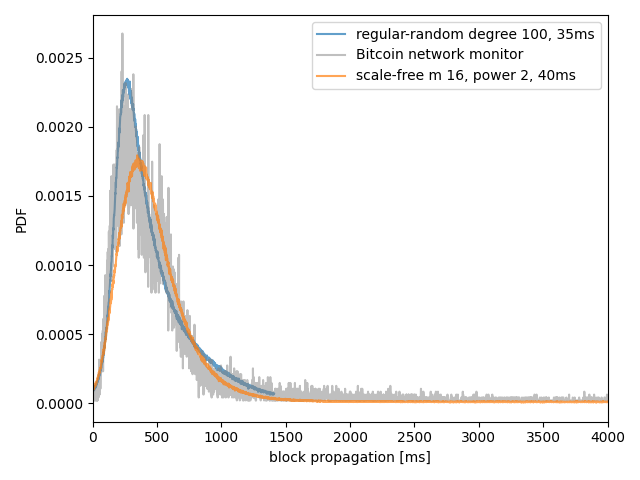
\includegraphics[width=\textwidth]{figures/propagation_histogram_withBitcoin.png}
		\caption{Selfish Rumor Model Model Block Propagation Distribution and Bitcoin}
		\label{fig:SRMBitcoin2}
	\end{subfigure}
\caption{Selfish Rumor Model Experiments in comparison with Bitcoin, 500 Peers}
\label{fig:SMRBitcoin}
\end{figure}

Figure~\ref{fig:SMRBitcoin} shows the most important results of various experiments carried out to minimize the RMSE between the simulations and Bitcoin. It also offers a comparison between the scale-free topology shown as orange and the regular random topology shown as blue. Since both topologies differ only in the degree distribution, we can compare both by their average degree respectively. All block delays were grouped in $1ms$ steps. All setups were repeated 100 times to ensure statistical significance.\\
Figure~\ref{fig:RMSE} shows the Root-Mean-Square-Error(RMSE) for 16, 32, 68, 100, 140 degrees and various communication process rates in comparison to Bitcoin. The lowest RMSE, $0.00016$, was achieved by 100-regular-random graph with a communication process rate of $35ms$. This parameter setup is referred to as $RegRan$. 
In Addition the results for a 16- and 32-regular-random graph are also shown in Figure~\ref{fig:RMSE}. A 32 degree regular random graph is used by \gopalan ~to evaluate against Bitcoin data. However, the RMSE-values are significantly higher than those of the 100-regular-random graph. This is most likely due to the usage of the FIBRE relay network and Compact Blocks in Bitcoin, which decreases block propagation delay. Additionally, all curves have a clear tendency towards a specific communication rate minimizing the RMSE.\\
This is also the case for scale-free networks, as is visualized in Figure~\ref{fig:RMSEBar}. For each topology there is one minimum communication rate, minimizing the RMSE against Bitcoin block propagation delay distribution. The scale-free network is generated over the Barabasi-Albert algorithm. This algorithm has three determining parameters. The number of vertices, $m$ for the number of edges generated for each vertex and a power factor. Since the lowest RMSE was always achieved for the power factor $2$ Figure~\ref{fig:RMSEBar} shows only the RMSE for power $2$.
The lowest achieved RMSE, $0.00018$, for scale free networks was for an average of 16 m, a power factor of 2 and a communication process rate of 40ms. This parameter setup is referred to as $ScaFre$.\\
Both topologies achieve quite low RMSE values. However, Figure~\ref{fig:minRMSE} visualizes the difference between the minimum RMSE values achieved for each average degree for both random regular and scale free graphs.
Regular random graphs lower the RMSE values for an increasing average degree, until an average degree of 80. Above an average degree of 80 the RMSE values remain quite constant.\\
The analyzation of parameter setups for scale free networks is more complex. Scale-free networks, in terms of the Barabasi-Albert model, have the parameter m, which can be used to control the average degree of the network. Additionally scale-free networks have a power factor, which controls the preferential attachment process. Since 4 different power factors were analyzed for each setup, Figure~\ref{fig:minRMSE} visualizes 4 datapoints above each other for each average degree. We can observe that for $m=16$ and for $m=32$ the achieved RMSE values are the lowest for power factor 2 and a communication process rate of 40ms.\\
Figure~\ref{fig:SRMBitcoin2} visualizes the block propagation distribution from the Selfish Rumor Model for both tested topologies in their minimum configuration and Bitcoin. The regular random graph models the peak closer. The scale free network cannot model the peak as good as the regular random network, but the curve shows more distinctly the longtail behavior. The better model for lower delays achieves a better RMSE value, since lower delays contain much more data points. Since data points above 1500ms are rare for Bitcoin, the exact modelling of the long tail does not impact the RMSE value as much. Nonetheless, both parameter setups are valuable to establish a validated Selfish Rumor Model Setup.\\
We conclude this section by establishing two parameter setups. The minimum configuration for regular random networks is called $RegRan$ and the minimum configuration for scale-free networks is called $ScaFre$. Both are discussed in their differences in the above chapter exhaustively. However, there are also
characteristics both share.
The interarrival time of the block arrival process is set to 600s. In a scenario, where multiple blocks could be transferred from one peer to another the block with the earliest arrival time is chosen. The number of peers is set to 500 and the mining power distribution is exponential. Additionally Simulations are always carried out 100 times to ensure statistical significance.\\
Those parameter setups, $RegRan$ and $ScaFre$ are used for following evaluations.

\section{Selfish Mining and Networking Effects}
Networking effects and selfish mining can be analyzed from a global and a local point of view, cf. Table~\ref{keyfactors}. The system analysis introduced by \gopalan assesses the system mainly in terms of consistency and blockchain growth, as discussed in the previous section. Both, blockchain growth and consistency, are influenced by adversarial mining strategies such as selfish mining. Additionally, selfish mining is influenced by networking factors.

\subsection{Selfish Mining in homogenous Network Setting}
\cauth{eyal} discovered a relationship between the relative computational power and the resulting revenue gain. They described that an increase in networking propagation factor and relative computational power results in an increased revenue gain. In a homogenous network every peer has the same degree and the same bandwidth. Such a network setup is the $RegRan$ setup and it can be used to analyze selfish mining in a scenario without any networking advantage.
\begin{figure}[h! t]
	 \begin{subfigure}[b]{0.48\textwidth}
		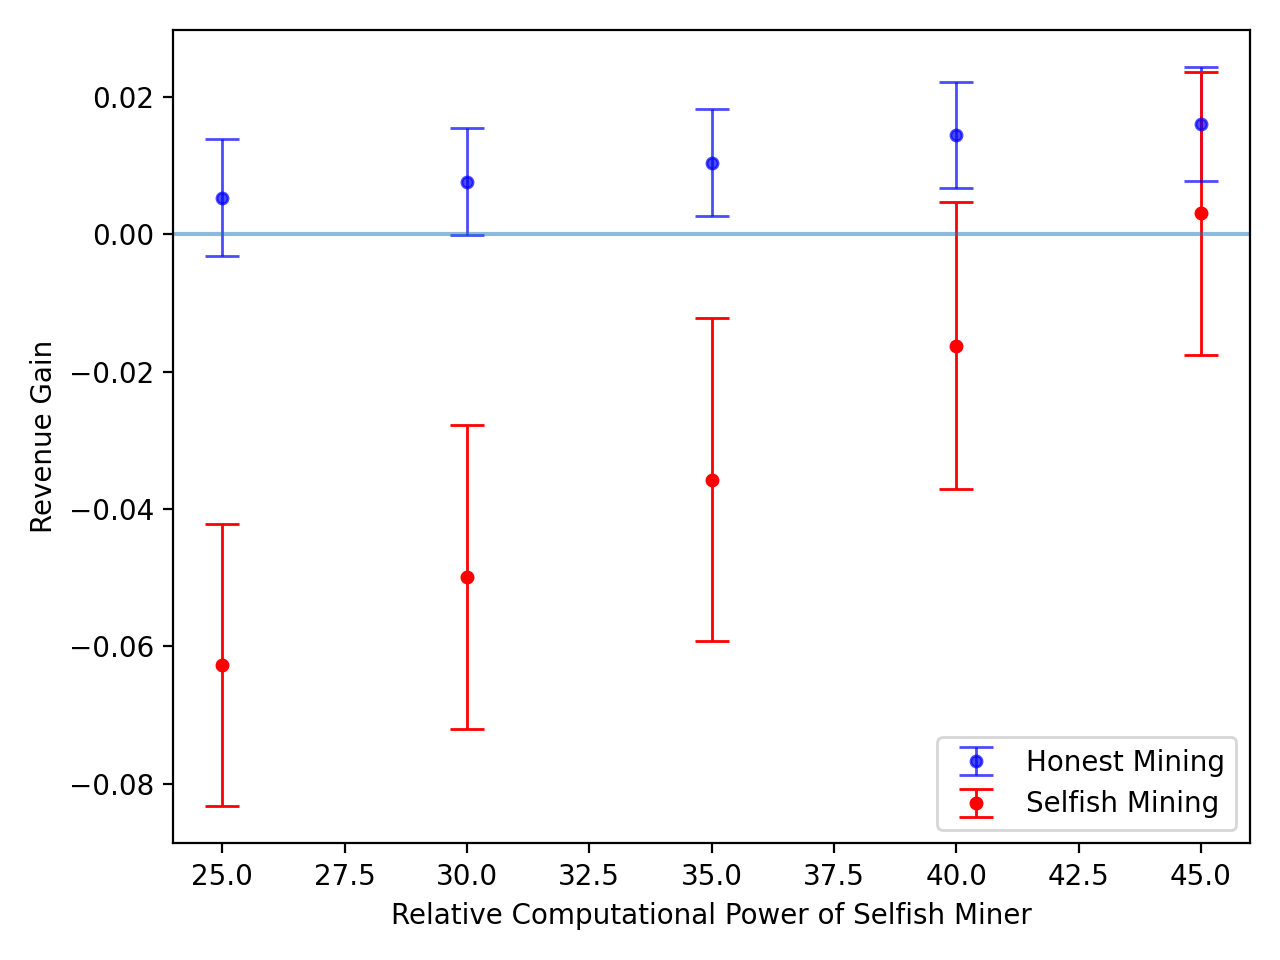
\includegraphics[width=\textwidth]{figures/rev_and_bpr_per_peer.png}
		\caption{Revenue and blockproduction\\ with standard deviation}
		\label{fig:multi_hr}
	\end{subfigure}
	\hfill
	\begin{subfigure}[b]{0.48\textwidth}
		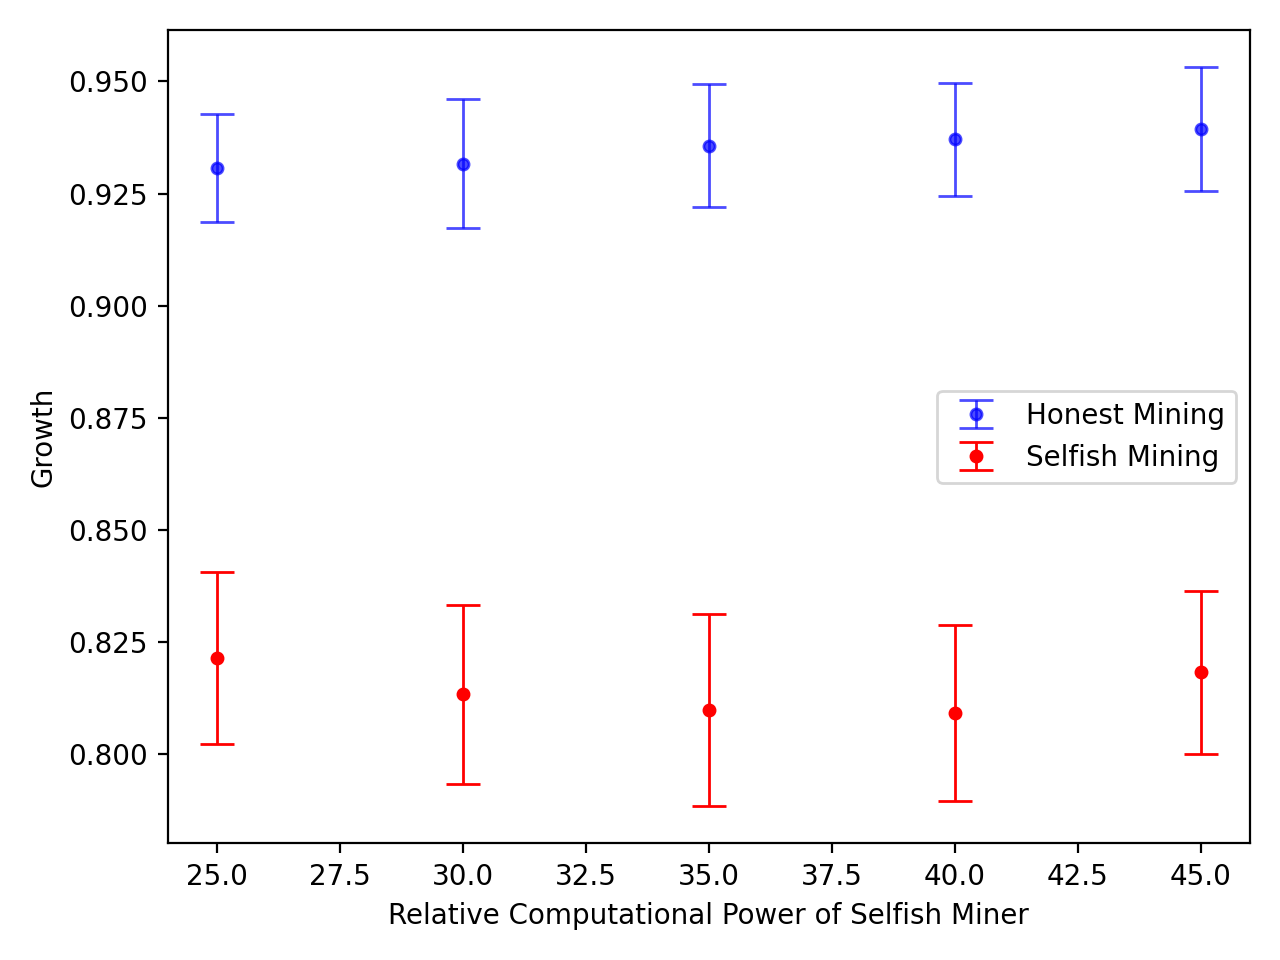
\includegraphics[width=\textwidth]{figures/growth.png}
		\caption{relative average growth of blockchain \\with standard deviation}
		\label{fig:multi_hr_growth}
	\end{subfigure}
	\caption{Simulations $RegRan$ Setup, multiple hashrates, Comparison between peer $0$ executing honest and selfish mining}
	\label{fig:mhr}
\end{figure}
Figure~\ref{fig:multi_hr} shows the revenue gain for relative compuational power between $25\% $ and $45\% $. Figure~\ref{fig:multi_hr} shows that for selfish mining the revenue gain is on average below zero except for $45\% $ relative computational power. For honest mining it is above zero. This shows that in this scenario honest mining is outperforming selfish mining. Increasing the relative computational power also increases revenue gain for the selfish miner. The small revenue gain of the honest miner increases as well, but only very slightly. The revenue gain has a greater standard deviation for the selfish miner than for the honest miner. Especially for the selfish miner revenue gain is wide spread. Nonetheless, the results contradict the \cauth{eyal} since the authors showed a strict revenue increase for $\alpha > 33\% $. Since $\alpha$ can be seen as the fraction of blocks a miner produces it is directly linked to the relative computational power this miner possesses. Thus, according to \cauth{eyal} Figure~\ref{fig:multi_hr} should be positive for the relative compuational power greater than $33\% $, which is very clearly not the case.\\
The overall growth of the blockchain is influenced by the selfish mining protocol, as is visualized in \ref{fig:multi_hr_growth}. Growth is the length of longest chain divided by the number of produced blocks. In an ideal case the growth of the blockchain is $1$ for a complete honest network. However, network effects result in a growth $~93\% $ even in a total honest network. This also explains the revenue gain of the honest miner. Since the blockchain contains fork a peer producing a large amount of blocks, will gain more revenue than its relative share. We can observe as well that selfish mining lowers the overall growth of the blockchain, as expected. For the setup containing the selfish miner the overall growth remains constant at around $82\% $. Note, that the growth reduction seems to be independent of the relative share of computational power the selfish miner possesses, at least for relative computational powers between $25-45\% $.\\
Selfish mining in an homogenous network setting does not result in a revenue gain compared to honest mining.

\subsection{Selfish Mining with Network Advantage}
Selfish Mining in a homogenous network is not beneficial. Therefore, analysis is conducted in network settings, where the selfish miner possesses a network advantage. 






\ifx
\newpage
\textcolor{red}{Ab hier, TODO}
\subsection{Selfish Mining with Networking Advantage}

topological advantage, and "bandwidth"

"trying to make selfish mining work"
\subsection{On Achievability of Networking Advantage}
betweeness centrality discussion
\subsection{Selfish Mining and Global Network Characteristics}
vllt das ans ende?	

mainly focus on growth? growth analyse war leider bisher etwas enttäuschend

This section will analyze how global system behavior changes when peers executing selfish mining are introduced to the system. In Section~\ref{gopalananalysis} the Simpy Blockchain Simulator was verified against the results published by \gopalan. \gopalan analyzed the blockchain system from a global perspective using metrices based on growth and block propagation. Thus, those base metrices will be first used to analyze the global state with adversarial miners.

\textcolor{red}{TODO: vgl. zwischen sm und nicht etc.}

Selfish mining leads to intentional forks in the blockchain.

  






\subsection{Networking effects impacting selfish mining}
Central to this thesis remains the question how impactful network effects are on the performance of selfish mining. The comparison of local and global factors from a single peer point of view can be utilized to describe a networking advantage this peer possesses.
Selfish mining is executed in order to gain revenue. Revenue gain can be measured by comparing the actual revenue to the relative computational power of the peer.
\subsubsection{Computational Power and Selfish Mining}


\subsubsection{Network Advantage and Selfish Mining}
Key aspects determining networking characteristics of a specific peer are his location relative to the network and his bandwidth, while key factors on a global scale are topology, network size and bandwidth distribution, as described in Table~\ref{keyfactors}. If for example all peers in the network possess the same amount of bandwidth, increasing the bandwidth of the selfish miner will put him at a network advantage.
If the network topology is described as a $k$-random regular graph, then allowing the selfish miner to connect to more then $k$ peers will result in a networking advantage. This topological factor can be measured by graph metrices, such as betweeness centrality.

\paragraph{Betweeness Centrality}
If revenue gain is positively correlated to network advantage, than a goal of a selfish miner should be to increase his network advantage. As discussed before one can analyze the resulting networking advantage utilizing network metrices such as betweeness centrality.
\begin{figure}[ht]
	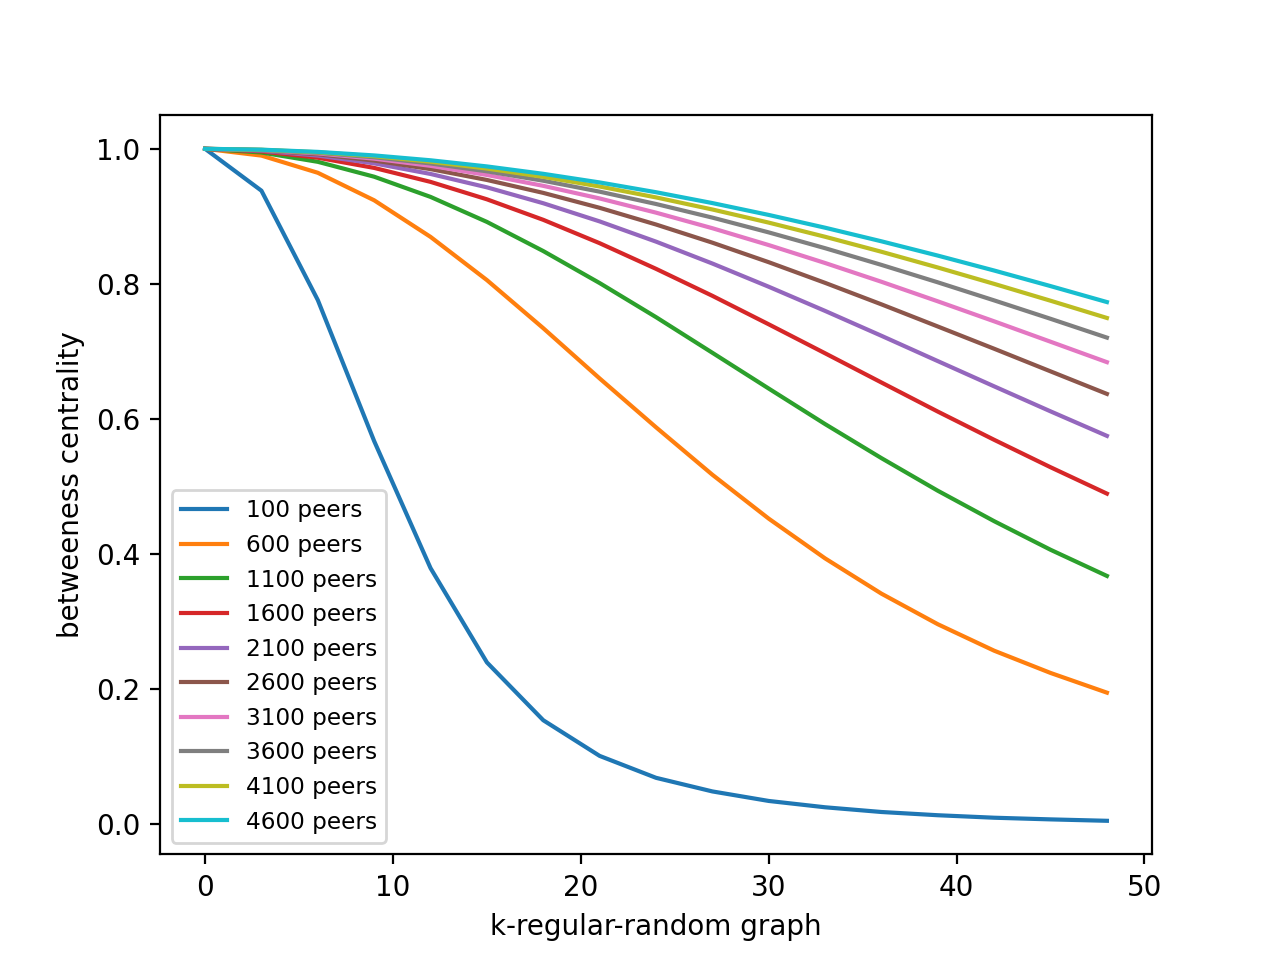
\includegraphics[width=\textwidth]{figures/betweeness_centrality.png}
	\caption{Betweeness centrality for various k-random-regular graphs for an all-connected peer $0$}
	\label{fig:bet_cent}
\end{figure}
Figure~\ref{fig:bet_cent} visualizes the betweeness centrality of one peer in various k-random-regular graphs. This specific peer, peer $0$, is connected to all other nodes. The rest of the graph follows a random-regular structure. The x-axis visualizes the increasing $k$ of the k-random-regular graph. As $k$ increases the betweeness centrality of peer $0$ decreases. For smaller node amounts the decrease is faster than for bigger node amounts. This is due to the absolut increase in $k$ since a 20-regular-random graph of 100 peers is better connected than a 20-regular-random graph of 1100 peers. Better connected means in this case it is closer to a fully connected graph. The closer the graph gets to being fully connected the more the central role of peer $0$ decreases, since the number of alternative paths between any other two peers rises. Nonetheless, Figure~\ref{fig:bet_cent} shows the upper limit for peer $0$. This means that in general a peer has to connect to a large amount of peers, compared to the network average in order to obtain any networking advantage.

\subsubsection{Topological Networking Advantage}
It can be assumed that a peer with a higher degree than the network average possesses a networking advantage. Thus, raising the degree of the selfish miner puts him at a topological networking advantage. We can then estimate the actual networking advantage based on the betweeness centrality and $\gamma$ of the peer. 
\begin{figure}[ht]
		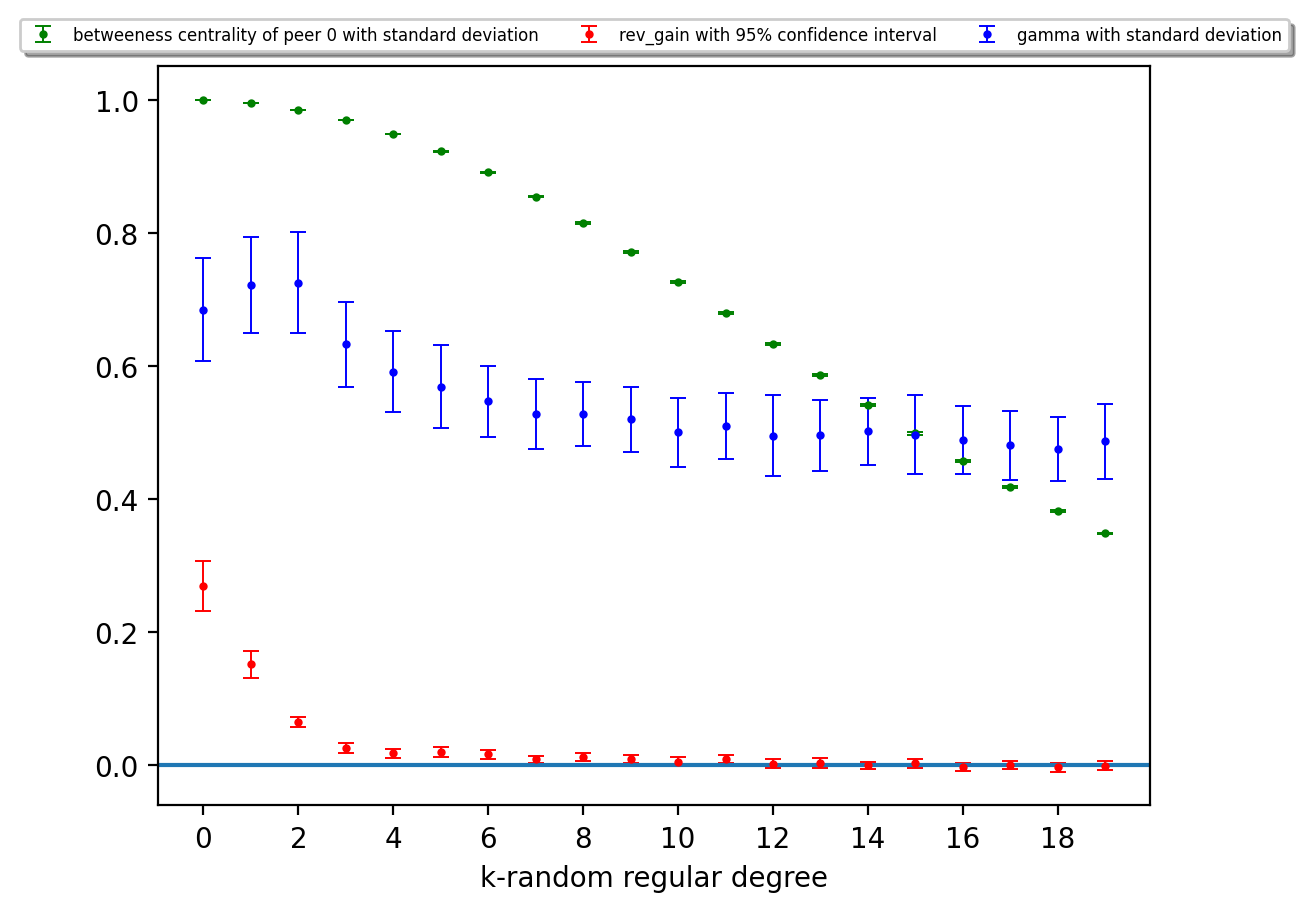
\includegraphics[width=\textwidth]{figures/full_sm_multi_degree_200rev_and_bpr_per_peer.png}
		
\caption{Betweeness Centrality, Revenue Gain and Network Propagation Factor, Topological Advantage Simulations with 200 Peers}
\label{fig:top_adv200}
\end{figure}

Figure~\ref{fig:top_adv200} shows results of experiments, which were based on analyzing the impact of topological network advantage. The experiments were carried out with 100, 200 and 300 peers respectively. Figure~\ref{fig:top_adv200} shows the results of the simulations for 200 peers, since no significant difference could be observed between 100, 200 and 300 peers simulations. The selfish miner possessed a relative computational power of $45\% $ while the rest was exponentially distributed on the remaining network. The interarrival time for communication process events was set to $1s$. The interarrival time for the block arrival process was set to $100s$. The selfish miner was connected to all peers. The rest of the network topology formed a $k$-random-regular graph, with an increasing $k$ shown in the x-axis.

The green bars represent the betweeness centrality of the selfish miner. The betweeness centrality of the selfish miner decreases as $k$ increases. The blue bar represents $\gamma$. We can observe that for each categroy of peer amounts $\gamma$ is slightly highest for $k \in \{0,1,2\}$ and is rather constant for $k>2$. $\gamma$  constant at around $0.55$ even though the betweeness centrality drops for increasing $k$'s. Thus, it is likely that $\gamma$ and  betweeness centrality are not correlated.

We can further observe that the revenue gain, shown in red, is highest for $k=0$. This is understandable since at $k=0$ the selfish miner can effectively eclipse every peer. The selfish miner is in total control over the information flow. For $k=1$ and $k=2$ revenue gain begins decreasing towards $0$ revenue gain. At $k=1$ and $k=2$ the selfish miner can still eclipse parts of the network but since overall connectedness increases, it becomes harder for the selfish miner to effectively eclipse every peer in the network. For $k>2$ revenue gain still seems to be slightly above $0$ which suggests that selfish mining is profitable.


\fi



















